\documentclass[12pt,a4paper]{article}

\usepackage[utf8]{inputenc}
\usepackage[T1]{fontenc}
%\usepackage[brazilian]{babel}
\usepackage{amsmath}
\usepackage{booktabs}
\usepackage{graphicx}
\usepackage{natbib}

\title{Ozônio em Nova York: um resumo de maio a setembro de 1973}
\author{Igor Garcia}
\date{\today}

\begin{document}

\maketitle

\section{Os dados}

% Item 2: origem, numero de observacoes e de ausentes
Os dados vem da base airquality.csv com 153 observacoes e NA: 37.

A Tabela~\ref{tab:resumo} traz a média mensal, e a
Figura~\ref{fig:dist} mostra a dispersão por trás dela.

\begin{table}[htbp]
  \centering
  \caption{Média mensal do ozônio e número de dias medidos.}
  \label{tab:resumo}
  \begin{tabular}{lrr}
    \toprule
    Mês & Média (ppb) & Dias medidos \\
    \midrule
    Maio      & 23,62 & 26 \\
    Junho     & 29,44 &  9 \\
    Julho     & 59,12 & 26 \\
    Agosto    & 59,96 & 26 \\
    Setembro  & 31,45 & 29 \\
    \bottomrule
  \end{tabular}
\end{table}

\begin{figure}[htbp]
  \centering
  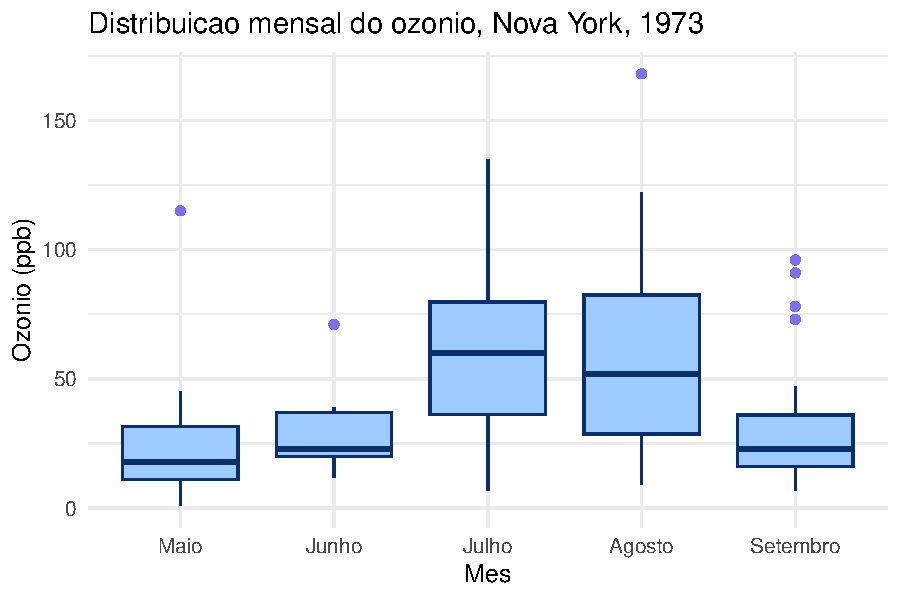
\includegraphics[width=0.8\textwidth]{figura.pdf}
  \caption{Distribuição do ozônio em cada mês.}
  \label{fig:dist}
\end{figure}

\section{O que os números dizem}

% Item 5: equacao numerada e a frase sobre o denominador
A média de cada mês é dada pela Equação~\eqref{eq:media}:

\begin{equation}
  \bar{x}_m = \frac{1}{n_m} \sum_{i \in M_m} x_i
  \label{eq:media}
\end{equation}

$n_m$ conta apenas
os dias em que houve medição, e não os dias do mês, de modo
que os ausentes reduzem o denominador em vez de entrarem
como zero.

% Item 6: as duas citacoes
A análise foi feita em R \citep{R2024} com o pacote
\texttt{ggplot2} \citep{ggplot2}.

\section*{Declaração de uso de IA}

% Item 7: obrigatoria, mesmo que a resposta seja "nenhuma"
Diga qual ferramenta usou, em que partes e como conferiu
o resultado.

\bibliographystyle{plainnat}
\bibliography{referencias}

\end{document}
